% calculus:x06 GDC:NO
\begin{question}
  \hspace*{\fill} [Note maximale: 16]\par
  \medskip
  \noindent La figure suivante représente une partie de la représentation graphique de $f(x) = 2x\sqrt[2]{a^2 - x^2}$,\par
  \noindent pour $-1 \le x \le a$, où $a > 1$\par
  \begin{center}
    \noindent La figure n'est pas a l'échelle\par
    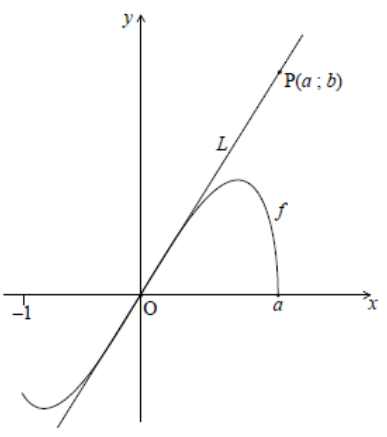
\includegraphics[scale=0.3]{temp_2xsqrtasq-xsq}\par
  \end{center}
  \medskip
  \noindent La droite $L$ est la tangente à la représentation graphique de $f$ à l'origine, $O$.\par
  \noindent Le Point $P(a; b)$ est sur $L$.\par
  \medskip
  (a)\par
  \hspace{1em}(i)  Étant donné que $f^\prime(x) =\frac{2a^2 - 4x^2}{\sqrt{a^2-x^2}}$, pour $-1 \le x \le a$,\par
  \hspace{2em} trouvez l'équation de $L$.\par
  \medskip
  \hspace{1em}(ii) À partir de là ou par toute autre methode, trouvez in l'expression pour $b$ en fonction de $a$\hspace*{\fill} [16]\par
  \medskip
\end{question}

